\documentclass[12pt,letterpaper]{article}
\usepackage[utf8]{inputenc}
\usepackage[T1]{fontenc}
\usepackage{float}

%% Sets page size and margins
\usepackage[a4paper,top=2.5cm,bottom=2.5cm,left=2cm,right=2cm]{geometry}

\usepackage{amsmath}
\usepackage{amssymb}
\usepackage{amsthm}
\usepackage{mathtools}
\usepackage{float}
\usepackage[colorinlistoftodos]{todonotes}

%Author affil
\usepackage{authblk}


%% Title
\title{
		\vspace{-0.7in} 	
		\usefont{OT1}{bch}{b}{n}
		\begin{minipage}{3cm}
        \vspace{-0.5in} 	
    	\begin{center}
    		
\includegraphics[height=3.2cm]{../logo_unam.png}
    	\end{center}
    \end{minipage}\hfill
    \begin{minipage}{10.7cm}
    
    	\begin{center}
\normalfont \normalsize \textsc{UNIVERSIDAD NACIONAL AUTÓNOMA DE MÉXICO \\ FACULTAD DE CIENCIAS \\ Organización y Arquitectura de Computadoras } \\
		\huge Tarea 01
    	\end{center}
     
    \end{minipage}\hfill
    \begin{minipage}{3.2cm}
    \vspace{-0.5in} 
    	\begin{center}
    		
\includegraphics[height=3.2cm]{../logo_fc.png}
    	\end{center}
    \end{minipage}

\author{Nieto Gallegos Isaac Julián}
\date{319021518}
}

 \setlength {\marginparwidth }{2cm}
 
\begin{document}

\maketitle

\textbf{Instrucciones:} Entregar por classroom en \LaTeX, escribir su nombre y número de cuenta en su tarea, la tarea es individual.\\

\begin{enumerate}
    \item Completa la siguiente tabla haciendo las conversiones necesarias. En los casos en la expresión después del punto se extienda, pueden acotarlo a solo 3 dígitos después del punto. (3 puntos).

    \begin{table}[H]
    \centering
    \begin{tabular}{|l|l|l|l|}
    \hline
    Decimal & Binario  & Octal & Hexadecimal \\ \hline
    20.3    & 10100.010& 24.231& 14.4CC      \\ \hline
    15      & 1111     & 17    & F           \\ \hline
    1.1     & 1.0001   & 1.060 & 1.199       \\ \hline
    10000   & 10011100010000& 23420 & 2710   \\ \hline
    3.125   & 11.001   & 3.1   & 3.2         \\ \hline
    1.5     & 1.1      & 1.4   & 1.8         \\ \hline
    17      & 10001    & 21    & 11          \\ \hline
    21      & 10101    & 25    & 15          \\ \hline
    2.34375 & 10.01011 & 2.26  & 2.58        \\ \hline
    4       & 100      & 4     & 4           \\ \hline
    1.125   & 1.001    & 1.1   & 1.2         \\ \hline
    63      & 111111   & 77    & 3F          \\ \hline
    10.75   & 1010.110 & 12.6  & A.B         \\ \hline
    6       & 110      & 6     & 6           \\ \hline
    55.375  & 110111.011 & 67.5& 37.6        \\ \hline
    10      & 1010     & 12    & A           \\ \hline
    18.789  & 00010010.11001010& 22.624& 12.CA \\ \hline
    367     & 101101111& 557   & 16F         \\ \hline
    1.0625  & 0001.0001& 1.001 & 1.1         \\ \hline
    3567.870& 110111101111.110111101111& 6757.6757& DEF.DEF     \\ \hline
    \end{tabular}
    \end{table}

    \item Contesta las siguientes preguntas, considera que 1kB y 1kb es diferente. (2 puntos).

    \begin{enumerate}
        \item ¿Cuántos bits hay en 36kb?


          Considerando que kb = kilobits entonces es inmediato que 36kb = 36,000 bits
        \item ¿Cuántos bytes hay en 24mb?


          Ya que 24mb = 24 megabits, entonces podríamos primero realizar la conversión y darnos cuenta que:

          $24mb = 24,000,000 b$.

          Luego entonces, dividimos esto por 8 pues cada byte equivale a 8 bits. Entonces: $24mb = 3,000,000 bytes = 3mB$
        \item ¿Cuál es el número más grande que se puede representar con 7 dígitos en base octal? (Escribelo en base 10 y en base 8)


          El número más grande de 7 dígitos en base octal es:

          $7777777$

          Que vendría a ser:
          \[7 * 8^7 + 7 * 8^6 + 7 * 8^5 + 7 * 8 ^4 + 7 * 8^3 + 7 * 8^2 + 7 * 8 + 7 = 2097151\]
        \item ¿Cuál es el número más pequeño y más grande que se pueden tener con el tipo uint16\_t de C?


          Este es un tipo entero, sin signo y de 16 bits. Es decir, es lo que conocemos como un unsigned short.

          Puede guardar hasta 16 bits de información y no lleva la limitación de llevar signo (por esto mismo su valor mínimo no es un negativo). Entonces puede ir de [0, 65535]

        \item ¿Por qué existen los tipos uint de C y cuáles son sus diferencias con otros tipos enteros como int o short?


          Un tipo uint es aquel que no guarda el bit más relevante para el signo del número, por lo que puede utilizar los n bits ($n = 32$ si es int, $n = 16$ si es short) para guardar toda la información del número.

          Esto se usa a costa de perder la capacidad de guardar números negativos, pues justamente perdemos la capacidad de darle signo a nuestros enteros.

          Se podrían utilizar para tener más espacio para guardar información de nuestro entero. Particularmente si lo usamos para esto, podemos guardar números dos veces más grandes de lo normal; pero por lo que investigué, esta práctica suele ser no recomendable.

          Generalmente se usan para aplicaciones en las que necesitamos manipular bits de manera más segura y previsible.

        \item ¿Cuántos bits se necesitan para poder direccionar todas las direcciones de una memoria de 500GB?


          Necesitamos entonces poder darle un número único (dirección) a cada uno de los bytes en estos 500GB de memoria. Primero consideremos que:
          \[500GB = 536,870,912,000 B\]
          Entonces necesitamos bits suficientes para representar un número mayor o igual a este.
          \[2^n \geq 536,870,912,000\]
          Aplicando logaritmo base 2 a este número obtenemos 38.965 aproximadamente.

          Luego esto lo redondeamos hacia arriba para tener holgura y entonces concluímos que necesitaríamos 39 bits al menos, para direccionar 500GB de memoria.

        \item ¿Cuántos dígitos en base hexadecimal se necesitan para representar un número en base binaria de 32 bits?


          Cada dígito hexadecimal puede representar 4 bits de una sola vez (pues puede representar 1-15). Entonces necesitamos 8 dígitos hexadecimales para representar 32bits

        \item ¿Quién o quiénes ganaron el premio nobel por la creación del transistor?


          John Bardee, Walter H. Brattain y William Shockley, en 1956

    \end{enumerate}


    \item  Escribe el siguiente circuito como una fórmula lógica y da su tabla de verdad. (3 puntos).
    \begin{figure}[H]
        \centering
        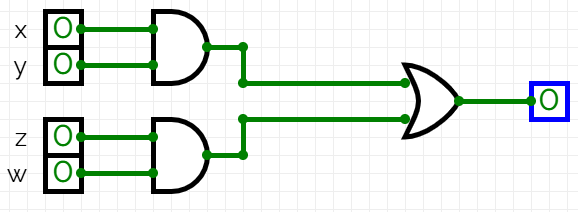
\includegraphics[width=0.75\linewidth]{circuito.png}
    \end{figure}

    Inmediatamente después de las entradas tenemos compuertas AND enlazando tanto x,y como z,w. Luego, estas mismas compuertas AND van hacia una compuerta OR.
    Entonces, la fórmula lógica sería: $(x\land y)\lor(z\land w)$.

    La tabla de verdad sería:
    \[
    \begin{array}{|c|c|c|c||c|c||c|}
      \hline
      x & y & z & w & x \land y & z \land w & (x \land y) \lor (z \land w) \\
      \hline
      0 & 0 & 0 & 0 & 0 & 0 & 0 \\
      0 & 0 & 0 & 1 & 0 & 0 & 0 \\
      0 & 0 & 1 & 0 & 0 & 0 & 0 \\
      0 & 0 & 1 & 1 & 0 & 1 & 1 \\
      0 & 1 & 0 & 0 & 0 & 0 & 0 \\
      0 & 1 & 0 & 1 & 0 & 0 & 0 \\
      0 & 1 & 1 & 0 & 0 & 0 & 0 \\
      0 & 1 & 1 & 1 & 0 & 1 & 1 \\
      1 & 0 & 0 & 0 & 0 & 0 & 0 \\
      1 & 0 & 0 & 1 & 0 & 0 & 0 \\
      1 & 0 & 1 & 0 & 0 & 0 & 0 \\
      1 & 0 & 1 & 1 & 0 & 1 & 1 \\
      1 & 1 & 0 & 0 & 1 & 0 & 1 \\
      1 & 1 & 0 & 1 & 1 & 0 & 1 \\
      1 & 1 & 1 & 0 & 1 & 0 & 1 \\
      1 & 1 & 1 & 1 & 1 & 1 & 1 \\
      \hline
    \end{array}
    \]

    \item Explica qué hace el siguiente código, qué se va a imprimir en la terminal y por qué. Puedes usar un compilador en línea de C para ejecutar el código. (2 puntos).
    \begin{figure}[H]
        \centering
        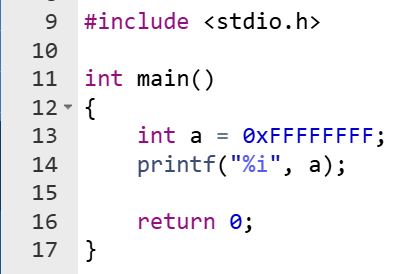
\includegraphics[width=0.5\linewidth]{image.png}
    \end{figure}
    Imprime el número máximo representable por 8 dígitos de hexadecimal; es decir, por 32 bits, que de hecho también es el tamaño de un valor entero en C

    Pero como estamos usando una variable entera con signo para guardar este valor, se estará guardando un número negativo en su complemento a dos. Es decir:

    Tenemos $11111111$, que es interpretado como un número negativo por ser entero con signo. Por lo que en complemento a dos esto es: $00000000 + 1 = 00000001 = -1$

    Entonces, esto imprimirá un -1 en pantalla
        
\end{enumerate}

\end{document}
